\documentclass{LTHtwocol} % Use this when you work on your report.
% \documentclass[final]{LTHtwocol} % Use this for the final version.
                                   % It will remove page numbers and
                                   % markers for overfull boxes.
                                   % There really shouldn't be any of those anyway.

\usepackage{subfiles}
\usepackage{caption}
\usepackage{subcaption}
\usepackage{multirow}
\usepackage{float}
\usepackage{graphicx}
\graphicspath{ {./resources/} }
\usepackage{adjustbox}
\usepackage{pgfgantt}
\usepackage{appendix}
\usepackage[subpreambles=true]{standalone}
\usepackage{import}
%\usepackage[backend=biber]{biblatex}
\usepackage[utf8]{inputenc}
\usepackage{graphicx,xcolor}
\usepackage{hyperref} 
\hypersetup{
  colorlinks,
  allcolors={blue!40!black},
}
\raggedbottom

\usepackage{kantlipsum} % Only for the dummy text. Remove for your own report.

\addbibresource{bibliography.bib}

% Document begins here
\begin{document}
\begin{frontmatter}
\title{Reinforcement Learning-Based Control of CrazyFlie 2.X Quadrotor} % Title of the project.
                      % Note that all reports are in English,
                      %so that our international students can read them.

\author[aj]{Arshad Javeed}
\author[val]{Valentín López Jiménez}

\email[aj]{ar1886ja-s@student.lu.se}
\email[val]{va7764lo-s@student.lu.se}

\advisor[johan]{Johan Grönqvist}
\email[johan]{johan.gronqvist@control.lth.se}

\begin{abstract}
The objective of the project is to explore synergies between classical control algorithms such as PID and contemporary reinforcement learning algorithms to come up with a pragmatic control mechanism to control the CrazyFlie 2.X quadrotor. The primary objective would be performing PID tuning using reinforcement learning strategies. The secondary objective is to leverage the learnings from the first task to implement control for navigation by integrating with the lighthouse positioning system. Two approaches are considered for navigation, a discrete navigation problem using Deep Q-Learning with finite predefined motion primitives, and deep reinforcement learning for a continuous navigation approach. Simulations for RL training will be performed on gym-pybullet-drones, an open-source gym-based environment for reinforcement learning, and the RL implementations are provided by stable-baselines3.
\end{abstract}

\end{frontmatter}
\section{Introduction}

Modeling a quadrotor such as CrazyFlie (figure \ref{cf:fig}) is not a straightforward task due to the non-linearities involved. Often, the system is linearized around a specific stationary point, but this is task-specific and could be daunting. Instead, we focus on a gray box approach, where we simulate our system using a physics engine \cite{pybullet_gym} to circumvent the physical modeling of the system.
In this paper, we synergize between classical PID control and reinforcement learning is explored to perform a navigation task in the CrazyFlie 2.X quadrotor. Pure classical or reinforcement learning approaches are not feasible in terms of convergence and are less interpretable. A pure RL approach demands a higher network architecture and long training hours to reach convergence. On the other hand, an end-to-end classical approach \cite{modelling_cf}\cite{nonlinear_control} controller's implementations can be complex as the design specification are not trivial.
 
In the research, first, we focus on PID tuning, where the parameters for the attitude and position Mellinger controller \cite{mellinger} are approximated using the Twin-Deep Deterministic Policy Gradient\cite{td3} algorithm and compared against the quadcopter's original values. Next, using the obtained PID parameters, a closed-loop controller is implemented in the simulation environment, where the quadrotor's task is to navigate to a determined point in space in a continuous environment. The RL agent is responsible for the high-level tasks and the PID loop executes the actions. Finally, robustness performance differences are explored in training with and without noise disturbances for the previous hovering navigation task.

 During the implementation of the RL tasks, the algorithm selected is TD3, from \verb|stable-baselines3| \cite{stable_baselines3}, considering its simplicity and robustness. We expect other more advanced actor-critic models to perform similarly.

\begin{figure}[H]
	\centering
	\caption{CrazyFlie 2.1}
	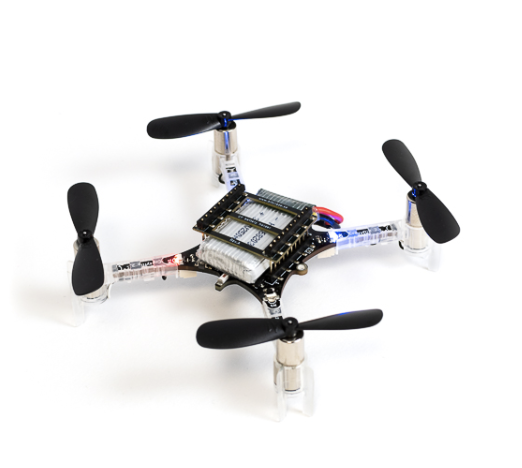
\includegraphics[scale=0.5]{cf.png}
	\label{cf:fig}
\end{figure}

\section{PID Tuning}
\import{sections/}{pid}

\section{Navigation}
\import{sections/}{nav}	

\section{Robustness}
\import{sections/}{robustness}

\section{Results}
\subsection{PID}
\import{sections/}{results_pid}

\subsection{Navigation}
\import{sections/}{results_nav}

\subsection{Roubstness}
\import{sections/}{results_rob}

\section{Conclusion}
\import{sections/}{conclusion}

\section{Acknowledgements}

We acknowledge our project advisors Johan Grönqvist and Emma Tegling for all the guidance and support. We would also like to acknowledge the Department of Automatic Control, Lund University for all the resources.

\newpage
\printbibliography

\onecolumn
\newpage

%\onecolumn
\section*{Appendix A: Software/Tools Used}

\begin{table}[H]
\label{app_a_software:table}
\centering
\begin{tabular}{|l|l|l|l|}
\hline
\textbf{Library}    & \textbf{Description}                                                                                                                        & \textbf{Version} & \textbf{License} \\ \hline
gym                 & A universal API for reinforcement learning environments                                                                                     & 0.21.0           & MIT License      \\ \hline
gym-pybullet-drones & \begin{tabular}[c]{@{}l@{}}PyBullet Gym environments for single and multi-agent\\ reinforcement learning of quadcopter control\end{tabular} & 0.0.3            & MIT License      \\ \hline
PyTorch             & \begin{tabular}[c]{@{}l@{}}Tensors and Dynamic neural networks in Python\\ with strong GPU acceleration\end{tabular}                        & 1.11.0           & BSD-3            \\ \hline
stable-baselines3   & \begin{tabular}[c]{@{}l@{}}Pytorch version of Stable Baselines, implementations of \\ reinforcement learning algorithms\end{tabular}        & 1.8.0            & MIT License      \\ \hline
cflib               & Crazyflie python driver                                                                                                                     & 0.1.22           & GPLv3            \\ \hline
\end{tabular}
\end{table}

%\onecolumn
\section*{Appendix B: Hardware}

\begin{table}[H]
\label{app_b_hardware:table}
\centering
\begin{tabular}{|l|l|l|}
\hline
\textbf{Hardware}          & \textbf{Description}                                                                                      & \textbf{Version} \\ \hline
CrazyFlie                  & Mini quadrotor                                                                                            & 2.1              \\ \hline
Caryradio                  & USB dongle for comm over radio                                                                            & 2.0              \\ \hline
Flow deck                  & Relative positioning system                                                                               & 2.0              \\ \hline
Lighthouse Deck            & Absolute positioning system                                                                               &                  \\ \hline
2 Lighthouse Base stations & \begin{tabular}[c]{@{}l@{}}Enables on-board positioning together\\  with the lighthouse deck\end{tabular} & 2.0              \\ \hline
\end{tabular}
\end{table}


%\section{Plan}
%
%\begin{ganttchart}[
%vgrid={draw=none, dotted},
%bar/.append style={fill=black},
%expand chart=\textwidth
%]{1}{11}
%    \gantttitle{Week}{11} \\
%    \gantttitlelist{1,...,11}{1} \\
%    \ganttbar[progress=100]{4.1.a: PID Tuning (Sim)}{1}{2} \\
%    \ganttbar[progress=100]{4.1.b: Demo 1: PID}{3}{3} \\
%    \ganttbar[progress=100]{4.2.d: Lighthouse Positioning}{3}{4} \\
%    \ganttbar[progress=100]{4.2.a: Env for Nav (Sim)}{4}{4} \\
%    \ganttbar{4.2.b: Discrete Problem (Sim)}{5}{6} \\
%    \ganttbar[progress=50]{4.2.c: Continuous Problem (Sim)}{5}{6} \\
%    \ganttbar[progress=0]{4.2.e: *** Explore AI deck}{10}{11} \\
%    \ganttbar[progress=50]{4.2.f: Demo 2: Comm over Radio}{7}{8} \\
%    \ganttbar[progress=25]{4.2.g: ** Robustness/Obstacle Avoidance}{8}{9} \\
%\end{ganttchart}

\end{document}